%--------------------------------------
% Master's Thesis Title Page
% LaTeX Template
% Version 1.0 (23/05/14)
%---------------------------------------

%----------------------------------------------------------------------------------------
%	PACKAGES AND OTHER DOCUMENT CONFIGURATIONS
%----------------------------------------------------------------------------------------

\documentclass[a4paper, 12pt]{report}
\usepackage{helvet}
\usepackage[toc,acronym,nomain]{glossaries}
\usepackage{graphicx} % Displaying pictures in the document.
\usepackage[floatrow]{chemstyle} % Displaying figures next to item lists.
\usepackage[hidelinks]{hyperref}
\usepackage{listings} % Adding source code listings.
\usepackage{caption}
\usepackage{algpseudocode}
\usepackage{subcaption}
\usepackage{color}
\usepackage[usenames,dvipsnames]{xcolor}
\usepackage{epstopdf}
\usepackage{gensymb}
\usepackage{mathtools}
\usepackage{courier}
\usepackage{fancyhdr}
 
\fancyhf{}
\rhead{\textbf{\thepage}}
\lhead{\textbf{\rightmark}}

\newglossaryentry{js} 		{ name=JavaScript,	description={A scripting language used in web development}}
\newglossaryentry{cpp} 		{name=C++, description={A object-oriented programming language.}}
\newglossaryentry{sc} 		{name=SystemC, description={A simulation library building on C++}}
\newglossaryentry{sampa}  {name=SAMPA, description={SAMPA ASIC}, plural=SAMPAs}
\newglossaryentry{vhdl}{name=VHDL,  description={A Hardware description language}}
\newglossaryentry{verilog}{name=Verilog, description={A Hardware description language}}
\newglossaryentry{altro}{name=ALTRO, description={ALTRO ASIC}}
\newglossaryentry{zs}{name=Zero Suppression, description={Suppression schema/algorithm}}
\newglossaryentry{pq}{name= Priority Queue, description={Datastructure which sorts elements based on a priority(numerical value)}}
\newglossaryentry{rng}{name= Random Number Generator, description={Computational device designed to generate numbers that lack a pattern}}

\newacronym{lhc}{LHC}{Large Hadron Collider}
\newacronym{cern}{CERN}{European Organization for Nuclear Research}
\newacronym{alice}{ALICE}{A Large Ion Collider Experiment}
\newacronym{tpc}{TPC}{Time Projection Chamber}
\newacronym{tev}{TeV}{Tera Electron Volt}
\newacronym{qcd}{QCD}{Quantum Chromodynamics}
\newacronym{asic}{ASIC}{Application Specific Integrated Circuits}
\newacronym{rcu}{RCU}{Readout Control Unit}
\newacronym{cru}{CRU}{Common Readout Unit}
\newacronym{gbt}{GBTx}{Giga Bit Transceiver}
\newacronym{fec}{FEC}{Front-End Card}
\newacronym{fifo}{FIFO}{First-In-First-Out}
\newacronym{gem}{GEM}{Gas Electron Multiplier}
\newacronym{mwpc}{MWPC}{Multi Wire Proportional Chamber}
\newacronym{fpga}{FPGA}{Field-Programmable Gate Array}
\newacronym{bt}{BT}{Binary Tree}
\newacronym{oop}{OOP}{Object-Oriented Programming}

\makeglossaries
\definecolor{mygreen}{rgb}{0,0.8,0}
\definecolor{mygray}{rgb}{0.5,0.5,0.5}
\definecolor{listinggray}{gray}{0.5}
\definecolor{lbcolor}{rgb}{0.95,0.95,0.95}

\newcommand{\codeword}[1]{\texttt{#1}}

% Solarized colour scheme for listings
\definecolor{variable}{RGB}{43, 145, 175}
\definecolor{keyword}{RGB}{0, 0, 255}
\definecolor{number}{HTML}{0080A0}
\definecolor{string}{RGB}{163, 21, 21}
\definecolor{comment}{RGB}{0, 128, 0}
\definecolor{background}{HTML}{FFFFFF}
\definecolor{function}{RGB}{111, 0, 138}

% Define C++ syntax highlighting colour scheme
\lstset{language=C++,
		backgroundcolor=\color{background},
        basicstyle=\footnotesize\ttfamily,
        numbers=left,
        tabsize=2,
        breaklines=true,
        escapeinside={@}{@},
        numberstyle=\tiny\color{black},
        keywordstyle=\color{keyword},
        stringstyle=\color{string}\ttfamily,
        %identifierstyle=\color{function},
        commentstyle=\color{comment},
       %directivestyle=\color{black},
        frame=single,
        rulecolor=\color{black},
        showstringspaces=false,
        captionpos=b
}
\DeclareCaptionFont{code}{\color{black}}
\DeclareCaptionFormat{listing}{ #1#2#3  }
\captionsetup[lstlisting]{ format=listing, labelfont=code, textfont=code, singlelinecheck=false, margin=0pt, font={bf,footnotesize} }

\lstnewenvironment{code}[1][]%
{
   \noindent
   \minipage{\linewidth}
   \vspace{0.5\baselineskip}
   \lstset{basicstyle=\ttfamily\footnotesize,frame=single,#1}}
{\endminipage}
%----------------------------------------------------------------------------------------
%	TITLE PAGE
%----------------------------------------------------------------------------------------

\newcommand*{\titlePage}{\begingroup % Create the command for including the title page in the document
\fontfamily{phv}\selectfont
\centering % Center all text

\vspace{200pt}
{\Huge SystemC simulation of the future SAMPA ASIC for use in the ALICE Experiment in Run 3} \\ % Title
\vspace{5pt}

{\Large \textsl{Consectetur adipisicing elit, sed do tempor incididunt ut labore et dolore magna aliqua}} % Subtitle or further description
\vspace{50pt}

{\Large{H\r{a}vard Rustad Olsen}}\\ % Author name

\vfill % Whitespace between the author name and the publisher logo

{\Large Master's thesis in Software Engineering at \\
\vspace{10pt}
Department of Computing, Mathematics and Physics, \\
Bergen University College \\
\vspace{10pt}
Department of  Informatics, \\
University of Bergen \\}
\vspace{10pt}
{\large June 2015} % Month and year published


\begin{figure}[h]
		\begin{subfigure}[]{50pt}
			
\includegraphics[width=50pt]{HIB_sort_hovedlogo.eps}
		\end{subfigure}
		\hfill
		\begin{subfigure}[]{50pt}
			
\includegraphics[width=50pt]{uib-logo.eps}
		\end{subfigure}

\end{figure}

\endgroup}

%----------------------------------------------------------------------------------------
%	BLANK DOCUMENT
%----------------------------------------------------------------------------------------

\begin{document}

\pagestyle{empty} % Removes page numbers

\titlePage % This command includes the title page

\newpage


\chapter*{Acknowledgements}
\addcontentsline{toc}{chapter}{Acknowledgments}

\paragraph{•}
Håvard Helstrup, Johan Alme, Dieter, Arild, Christian, (Damian).
\newpage

\phantomsection
\addcontentsline{toc}{chapter}{Contents}
\tableofcontents

\newpage
\phantomsection
\addcontentsline{toc}{chapter}{List of Figures}
\listoffigures

\newpage
\phantomsection
\addcontentsline{toc}{chapter}{List of Tables}
\listoftables

\newpage
\phantomsection
\addcontentsline{toc}{chapter}{Listings}
\lstlistoflistings
\newpage

% Glossary
%\chapter*{Glossary and acronyms}
%\addcontentsline{toc}{chapter}{Glossary and acronyms}
\printglossaries
\newpage
\pagestyle{fancy}
\chapter{Introduction}
\textit{This chapter will cover the motivation, as well as the scope and goal of this report.}

\section{Motivation}
\label{sec:motivation}
\paragraph{•}
The \gls{lhc} at the \gls{cern} is the world's largest particle accelerator, hosting multiple ongoing experiments.
After a run period of more than 3 years, the \gls{lhc} will be shut down from 2018 until 2021.\cite{ls2}
The purpose of this shutdown is to do maintenance on various equipment in the \gls{lhc}, as well as significant upgrades to the different detectors, one of which is the detector for the \gls{alice}.
\gls{alice} consists of multiple sub-detectors, which combined collect an enormous amount of data.
This amount is expected to increase after the shutdown period as the interaction rate of the \gls{lhc} will increase.
Due to the increase in data output, the \gls{alice} collaboration is seeking to upgrade and enhance the detector capabilities.\cite{alice-upgrade}
This includes a partial redesign of the readout electronics, upgrades to multiple sub-detectors and additional hardware upgrades.

\paragraph{•}
The \gls{tpc} is the \gls{alice} detector's main sub-detector for tracking and identifying particles.
A starting design for the new \gls{tpc} readout electronics has been made, and the different components are currently being developed.
As this is still being worked on, many questions about the different components are yet to be answered.
Are the current specifications sufficient to handle the expected increase in output from the detector?
Do they have the necessary bandwidth to be able to send the data with minimal sample loss.
Are the buffer memory enough to handle the traffic.
Is it possible to optimize the current solution in any way?

\paragraph{•}
The previous paragraph provides motivation for us to find a reliable way of determining a sufficient design for the readout electronics, while being both time and cost efficient.
One strategy for solving this problem, which will be further explored in this thesis is creating a simulation of the system.
Doing a simulation requires designing a accurate representation of the readout electronics, and creating a testbench where it is possible to configure and run multiple tests.


\section{Research Question and thesis goal}

\paragraph{•}
Given the motivation and introduction given in section \ref{sec:motivation} the research question for this thesis becomes:

\paragraph{•}
Is it possible to design and implement a simulation which directly represent the readout electronics, and in doing so will it have an optimizing effect?

\paragraph{•}
Further explained, the main tasks of this thesis will be to create a computer model of the readout electronics main components, and run multiple simulations on it.
Experimenting with different configurations in order to find bottlenecks, faulty design or areas of improvement.
The experiments should be logged, and the results will be presented in an organized fashion.


\section{Report structure}
Chapter 2 will give the reader the background information to be able to understand the different academic and scientific terms used, as well as some information about the context of the report.
This includes information about \gls{cern}, the \gls{alice} experiment and the physics most relevant to the thesis.
It will discuss the current readout electronics as well as the proposed upgrade.
Chapter 3 is going further into the problem discussed in this report, initial plans on solving the problem, and information about the tools used.
Chapter 4 will talk about the implementation of the simulation, what problems occurred along the way, and the chosen solution.
The chapter will go into the design, as well as code snippets from the implementation.
With the information given in chapter 4, chapter 5 will discuss the results of the different simulation runs, and evaluate the solution.
Chapter 6 will conclude the thesis with some closing words, and work that can be done in the future.


\chapter{Background}
\textit{This chapter will give the reader the background needed to set the rest of the thesis in context.}

\section{CERN}
\paragraph{•}
\gls{cern} is a European research and scientific organization based out of Geneva near the Franco-Swiss border\cite{cern}.
\gls{cern} is a collaboration between 21 countries with a member staff of over 2500, and more than 12000 associates and apprentices.
The organization was founded in 1954 and has since then been the birthplace of many major scientific discoveries.
These are not limited to discoveries in the field of physics, but includes the creation of the World Wide Web\cite{www}.
Currently the biggest project at \gls{cern} is the \gls{lhc} particle accelerator, which serves as the foundation for multiple experiments in the field of particle physics.
% 2 - 3 more sentences about this!

\section{The Large Hadron Collider}
\label{sec:lhc}
\paragraph{•}
Starting up on 10 September 2008, \gls{lhc} is the latest construct added to \gls{cern}'s particle accelerator complex\cite{lhc}.
It consist of a 27 kilometer underground ring of superconducting magnets which boost the energy of the particles travelling inside the collider.
The collider contains two adjacent parallel high-energy particle beams.
These beams consist of protons extracted from standard hydrogen atoms by stripping them of electrons.
Along the collider ring there are four intersection points where collisions occur.
Each point corresponds to the location of a particle detector - ATLAS, \gls{alice}, CMS and LHCb.
The particle detectors are each built and operated by large collaborations, with thousands of scientists from different institutes around the world.
The beams travel at close to the speed of light and are guided by magnetic fields, which are created and maintained by superconducting electromagnets.
Superconducting meaning that it is in a state where it can most efficiently conduct electricity, without resistance or energy loss.
Achieving this state requires cooling the magnets to -271.3\degree~C , which is done by the distribution of liquid helium.
The layout of the \gls{lhc} ring as well as its four collision points can be seen in \ref{fig:lhc}.

\begin{figure}[h!]
  \centering
    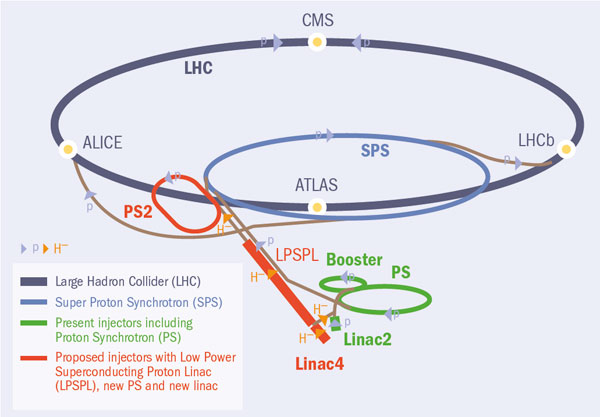
\includegraphics[width=0.7\textwidth]{images/lhc-ring.jpg}
     \caption{The Large Hadron Collider \cite{lhc-ring-image}}
    \label{fig:lhc}
\end{figure}

\paragraph{•}
The beams travelling inside the \gls{lhc} reach an energy-peak of 7 \gls{tev}, which means that on impact with each other the collision reach an energy of 14 \gls{tev}\cite{lhc-pdf}.
During a normal run of the collider there will be about 600 million particle collisions per second during a period of 10 hours.
This leads to a huge amount of data for each of the detectors to read out.
\gls{alice} is the detector which produce the most data per collision, with a design value of about 1.25 GB/s written to permanent storage.
The high amount of data per collision is produced primarily by the \gls{tpc} sub-detector, which records a high number of points per track, and has a low momentum threshold. Detectors like ATLAS and CMS  are designed with a higher momentum threshold, but can cope with significantly higher collision rates than ALICE.
ALICE is designed for the study of heavy ion reactions, where particle correlations at low momentum is an important measure.
The number of tracks correlating with momentum is exponentially declining.
This means that a lot of tracks which doesn't get registered in ATLAS, produces data in \gls{alice}.

\section{ALICE}
\subsection{Introduction}

\paragraph{•}
\gls{alice} is designed as a heavy-ion detector, which means it studies collisions between heavy nuclei of high energy\cite{alice-home}.
The experiments is run with two different particle collision systems, lead-lead(Pb-Pb) and lead-proton(Pb-p)
Both systems produce a extreme amount of temperature and density.
They produce different, but equally interesting results.
Pb-Pb collisions create Hot Nuclear Matter, while Pb-p create Cold Nuclear Matter.
The explanations for these types of matter is beyond the scope of this thesis and will not be discussed further.
The high temperature and density is necessary to produce a phase of matter called quark-gluon plasma.

\subsection{Quark-gluon plasma}
\paragraph{•}
Shortly after the Big Bang, the universe was filled with a extremely hot cluster of all kinds of different particles moving around at near the speed of light\cite{alice-physics}.
Most of these particles were quarks, fundamental building blocks for matter, and gluons which ties quarks together in order to form heavier particles.
Normally quarks and gluons are very strictly tied together, but in the conditions of extreme temperature and density as in the time shortly after the Big Bang, they are allowed to move freely in an extended volume called quark-gluon plasma.
The existence of quark-gluon plasma and its properties is one of the key issues in \gls{qcd}.
The \gls{alice} collaboration studies this, observing how it behaves.

\subsection{The detector setup}
\paragraph{•}
The detector weight is about 10,000 ton, it is 26 m long, 16 m wide, and 16 m high\cite{alice-about}.
It consists of 18 sub-detectors, each with its own set of tasks regarding tracking and identifying particles.
This large number of sub-detectors are needed in order to get the full picture of the complex system which is being studied(i.e different types of particles and the correlations between them).
Most of the detector is embedded in a magnetic field, created by a large solenoid magnet, which makes particles formed in collision bend according to their charge, and behave differently relative to their momentum. High momentum equals near straight lines while low momentum makes the particles move in spiral-like tracks.
During lead to lead collisions the collision rate peaks at 8 kHz(Where Hz is defined as number of events per second).
The number of recorded events is smaller in practice because the \gls{alice} detector uses a triggered readout, which only triggers on head-on(central) collisions.
The maximum readout rate of the current \gls{alice} detector is 500 Hz, which is more than enough to track central collisions.
\ref{fig:alice} shows a cross section of the detector as it is today with the red solenoid magnet, and all sub-detectors labeled.

\begin{figure}[h!]
  \centering
    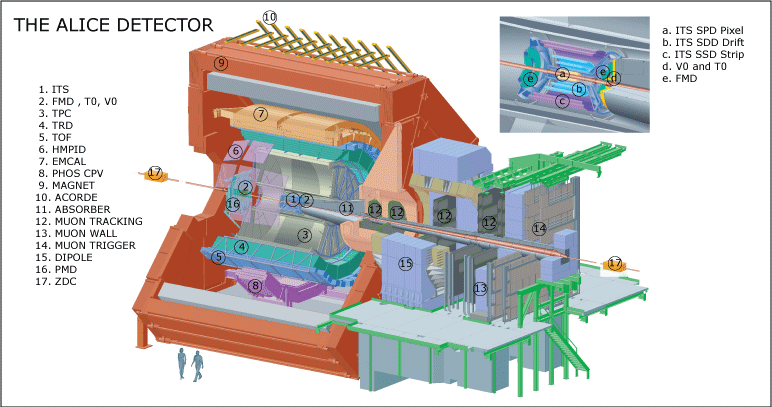
\includegraphics[width=1.0\textwidth]{images/alice-detector.png}
     \caption{The ALICE detector \cite{alice-image}}
    \label{fig:alice}
\end{figure}

\section{The TPC detector}
\subsection{Intro}
\paragraph{•}
One of the most important sub-detectors, and the one that is relevant for this thesis is the \gls{tpc} detector.
Located at the center of the \gls{alice} detector it is among the first entry points when gathering data from a particle collision.
It is a 88\(m^3\) cylinder filled with gas.
The gas works as a detection medium, which means that charged particles from a collision crossing will ionize the gas atoms, freeing electrons that move towards the end plates of the detector.
The readout is done by specially designed readout chambers, which are capable of handling the high amount of data produced in heavy-ion collisions.

\subsection{Readout electronics} %Should this be a chapter of itself?
\paragraph{•}
Signals from the readout chambers are passed along to the front-end readout electronics, which today consist of 4356 \gls{altro} \gls{asic} chips\cite{altro}.
\gls{asic} is the term used for specially customized chips, rather than chips with a more general-purpose use\cite{asic}.
The \gls{altro} chip is made up of 16 asynchronous channels that digitize, process and compress the analogue signals from the readout chambers.
It operates on a so called triggered readout mode.
In short when \gls{altro} receives the first trigger, it stores the following data stream into memory, holding on to it until it is ready to pass on the data.
The front-end electronics are able to readout data at a speed of up to 300 MB/s.
\paragraph{•}
The \gls{altro} chip sends the digitized signals further down the readout chain to the \gls{rcu}, where it is further processed and shipped to  and stored in the online systems.
The schematics is shown in \ref{fig:altro}.

\begin{figure}[h!]
  \centering
    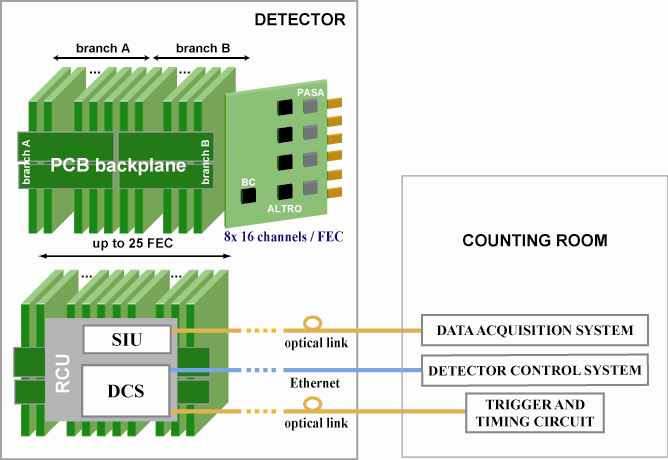
\includegraphics[width=0.75\textwidth]{images/altro.png}
     \caption{Readout schematics for the current TPC detector \cite{tdr-016}}
    \label{fig:altro}
\end{figure}

\section{Long Shutdown 2}
\paragraph{•}
As mentioned in \ref{sec:motivation} the \gls{lhc} ring will be shut down for about 3 years, starting 2018.
During that time the \gls{alice} detector will undergo an extensive upgrade.
The upgrade strategy for \gls{alice} is based on the expected increase in collision rate to 50 kHz, and will now track every collision.
Essentially this comes down to a increase by a factor of 100, compared to what is achievable today.

\paragraph{•} 
To be able to handle the increase in collision rate the \gls{tpc} will receive upgrades to both its readout chambers, and front-end readout electronics.
The current \gls{mwpc} based read-out chambers will be replaced by \gls{gem} detectors, which has a much higher readout rate capability.
Signals will be passed from the new readout chambers to the \gls{fec} via a readout pad structure similar to the one presently used, where each pad is mapped to a \gls{sampa} channel.
There are multiple pad structures depending on its location on the detector, but the difference in structure is not relevant for this thesis.
What is relevant however is that more data is expected from low pad numbers, an example of a pad structure is shown in \ref{fig:pad-struct}.

\begin{figure}[h!]
	\centering
		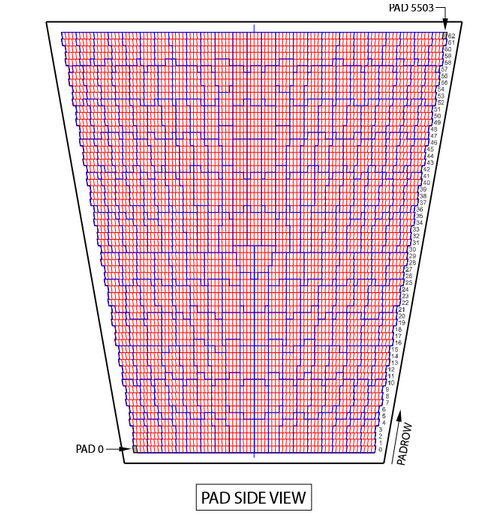
\includegraphics[width=0.75\textwidth]{images/pad-structure.png}
		\caption{Pad structure of an Inner Readout Chamber(IROC)\cite{pad-structure}}
		\label{fig:pad-struct}
\end{figure}

\paragraph{}
The entry point in the \gls{fec} is the new custom-made \gls{asic}, the \gls{sampa}, which will replace the \gls{altro} chip\cite{tdr-015}.
The \gls{sampa} chip is capable of processing signals asynchronously in 32 individual channels, each channel is directly connected to a single pad.
They are further on digitized and concurrently transferred to the \gls{gbt}, which enhances the signal strength and transmits them via multiple optical fiber links to the \gls{cru}.
The \gls{cru} can be thought of as the new \gls{rcu} and serves as an interface to the online systems.
The data flow from the detector, and a working schematics can be seen in \ref{fig:fec}.
Chapter~\ref{cha:4} will go into more detail about the readout electronics in the context of our simulation.

\begin{figure}[h!]
	\centering
		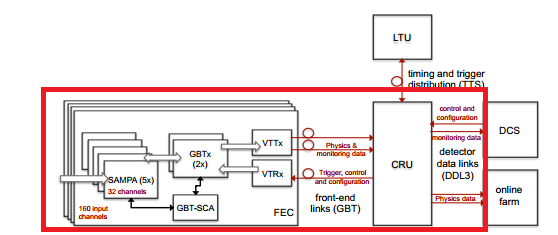
\includegraphics[width=0.75\textwidth]{images/fec.png}
		\caption{Schematics of the readout electronics \cite{tdr-016}}
		\label{fig:fec}
\end{figure}

\chapter{Simulations}

\textit{SystemC, Starting design of the simulation, plans for implementation and test runs}

\section{Simulation Theory}

\subsection{Theory}
\paragraph{•}
A simulation can be seen as the imitation of a real-world system and its operations over time.
This requires a model representation of the system which is accurate enough to conduct experiments on, which produce real-like results.
The model should include key characteristics, specifications and functions of the selected system, but in a simplified fashion.
A simulation model can take many forms as it can be used in different contexts ranging from physical object such as electrical circuits, bridges, and even entire cities to abstract systems like a mathematical equation or a scientific experiment\cite{simulations}.

\paragraph{•}
As the model represent the system itself, the simulation represents its operations over a set period of time.
The simulation is normally conducted in a controlled environment that makes it possible to observe, monitor and log results.
To achieve efficient experiments using a simulation, it should be easy to change its parameters with respect to what is being tested.

\paragraph{•}
There are many benefits of simulating a system instead of creating and test the real thing.
A simulation will in most cases be very time efficient, you can conduct the same kinds of experiments on the system in a much shorter time compared to the real thing.
This means that more information about the systems behavior and its limitations can be gathered in less time, which in turn can result in a better final product.
Creating the real-world system can often be very expensive, which may limit the amount of prototypes or test-products that are possible to create.
Therefore using results of a simulation to fine tune the specifications before starting to produce prototypes will cut unnecessary development costs by a significant margin.

\paragraph{•}
Taking the upgrade of the readout electronics for the \gls{alice} detector as an example to further address this point one can see the usefulness of not having to create multiple custom hardware components, all with different purposed specification.
In regards to the readout electronics, another important point is that the proposed designs might already function properly, but there is always room for improvement.
Finding out that the design doesn't need as much memory, or less optic fiber cables can impact the overall production costs.
One way to efficiently and accurately simulate hardware components is by creating a virtual computer simulation.

\subsection{Computer Simulations}
\paragraph{•}
Using computers to do simulations becomes more and more useful because of their incredible computational power, and ability to produce fast results.
This is important as simulations often become quite complex, both in regards to computational complexity and level of difficulty to understand and further work with.
Therefore it can be wise to use existing tools to help make the process easier.
There is an array of different tools that can be used to various kinds of simulations.
They vary from complete frameworks, with graphical user interfaces to tools which help programmers write there own simulation programs.
The later requires of course the most work, but will most often end with the better results as you can tailor your simulation on a lower level than with a complete framework.
A programming tool that is made for creating simulations is the \gls{sc} library, which will be discussed in the following section.

\section{SystemC}
\textit{Explain how SystemC works, what benefits and downsides}

\subsection{Background}
\paragraph{•}
\gls{sc} is a system design library based on \gls{cpp}\cite{systemc}.
It provides an interface to easily create a software model that represents a hardware architecture, and together with standard \gls{cpp} development tools it is possible to quickly build a full scale simulation.
Following the standards of \gls{cpp}, \gls{sc} is built to be easy to understand for both software and hardware developers, resulting in clearer cooperation between them while developing the hardware design.
The \gls{sc} library provides an object-oriented approach to model design, where a single \gls{cpp} class represents a model.
This makes it easy to separate concerns between the different models in your simulation.

\paragraph{•}
When simulating a hardware system there is a couple of key points to be aware of, firstly you need to be able to handle hardware timing, clock cycles, and synchronisation.
One of the benefits of \gls{sc} is that it takes care of all of this, again taking advantage of the object-oriented nature of \gls{cpp} to extend its capabilities through \codeword{classes}.
Here is some of the other features \gls{sc} provides, with emphasis on the ones needed to understand code snippets shown in this thesis.

\paragraph{•}
\begin{itemize}
\item \textbf{Modules}
	\begin{itemize}
		\item Container \codeword{class} representing a hardware model.
	\end{itemize}
\item \textbf{Processes}
	\begin{itemize}
		\item In short, processes are methods inside a module which describe the module functionality.
	\end{itemize}
\item \textbf{Ports}
	\begin{itemize}
		\item Ports represent the input and output points of a module, they can be connected to other modules through Channels.
		When you declare a port in a simulation, it is required to specify if the port is an input, output or bidirectional port.
		This is done by specifying a channel interface for the port.
		Example of a port using a input \gls{fifo} interface: \begin{verbatim}sc_port<sc_fifo_in_if>\end{verbatim}.
	\end{itemize}
\item \textbf{Channels}
	\begin{itemize}
		\item Channels are the wires connecting two Ports.
		\gls{sc} comes with three predefined channels: \gls{fifo}, mutex, and semaphore.
		It is possible to configure custom channels, but in most cases it is not necessary.
	\end{itemize}
\item \textbf{Signals}
	\begin{itemize}
		\item Signals represent data sent between modules via ports.
		They can be arbitrary data types like \codeword{bool} or \codeword{int}, but also user defined types.
	\end{itemize}
\item Rich set of data types
	\begin{itemize}
		\item \gls{sc} supports all data types defined in \gls{cpp} as well as multiple custom types.
	\end{itemize}
\item Clocks
	\begin{itemize}
		\item \gls{sc} comes with clocks, which can be seen as timekeepers of the system during a simulation.
	\end{itemize}
\end{itemize}

\newpage
\subsection{Small example}

\paragraph{•}
To get a basic understanding of how a \gls{sc} simulation looks like, it is useful to see it in action.
The following \ref{fig:sc-ex} and Listings~\ref{lst:prod-ex}-\ref{lst:main-ex} make up a very trivial example with only 2 modules; a \codeword{Producer} and a \codeword{Consumer}.
The \codeword{Producer} will increase a counter every clock cycle, and send a \codeword{bool} value based if the count is an even number, and send this value to the \codeword{Consumer}, which registers how many times the \codeword{Producer} counted an even number.
The example uses a \gls{fifo} channel, connected between an output port on the \codeword{Producer}, and an input port on the \codeword{Consumer}.

\begin{figure}[h!]
  \centering
    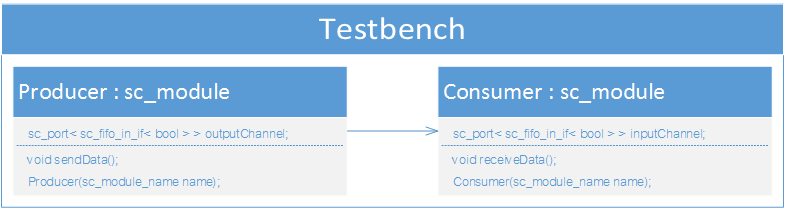
\includegraphics[width=1.0\textwidth]{images/sc-example.png}
     \caption{Basic SystemC example}
    \label{fig:sc-ex}
\end{figure}

\noindent
\begin{minipage}{\linewidth}
\lstinputlisting[caption=Producer module.,label=lst:prod-ex]{codelistings/producer.cpp}
\end{minipage}
\begin{minipage}{\linewidth}
\lstinputlisting[caption=Consumer module.,label=lst:cons-ex]{codelistings/consumer.cpp}
\end{minipage}
\begin{minipage}{\linewidth}
\lstinputlisting[caption=Simulation test-bench.,label=lst:main-ex]{codelistings/main.cpp}
\end{minipage}

\paragraph{}
\gls{sc} can be used to create very low level hardware descriptions and models, and can interface directly with hardware description languages like \gls{vhdl} and \gls{verilog}.
This is one way to create a simulation, and the models will be very accurately represented by doing so.
The other way is to have a high level of abstraction, leaving out the unimportant details and focus solely on the expected problem areas.
There are benefits and drawbacks for both ways, but sticking to a high abstraction level can in complex cases make it a lot easier to work with the model design and allows you to focus on the important parts.

\chapter{Problem Description}
\textit{Explain the model, introduce the problem}
\label{cha:4}

\paragraph{}
The previous chapters has briefly introduced the problems of this thesis, relevant background information and looked at tools and the method of solving them.
Essentially it boils down to creating a model based on the schematic of the \gls{tpc} readout electronics, run multiple simulations, testing different parameters for the involved components.
Until now there has only been an introduction level description of the different components that is being included in the simulation model.
This chapter will go deeper into them, giving detailed information about their design parameters, and how the \gls{alice} experiment data is handled by them.
Not going too far into the task of implementing this in a \gls{sc} environment, but focus on the different problem areas, what is required in order to solve them and what goals to achieve.

\section{Model Design}
\textit{Different design patterns, and plans for the electronics}
\paragraph{}
The hardware design which is being simulated is already briefly shown in \ref{fig:fec}.
The proposed schematic shown there consists of 12 \gls{fec} cards for every \gls{cru}.
Each \gls{fec} consists of 5 \gls{sampa} and 2 \gls{gbt} \glspl{asic}, with the \gls{cru} being connected to them via 24 optical links.
Out of the 3 main chips, the \gls{sampa} and the \gls{cru} are the most interesting as they are still being developed and testing them can give a lot of valuable feedback.
The \gls{gbt} is a completed component, so even though it is part of readout electronic being simulated, it will only be a very shallow abstraction of it.
This means that it will remain as an empty module whose objective will be to just pass along received data to the correct output links.
One important note about the \gls{gbt} input and output links.
Each \gls{gbt} has 10 input e-links, each with a transfer rate of 320 Mbit/s, giving an effective input speed of 3.2 Gbit/s per \gls{gbt}.
The output is 1 optical fiber link with a speed of 3.2 Gbit/s, giving the \gls{gbt} the same input and output speed.
This is the reason letting data flow directly through the \gls{gbt} in the simulation is possible.
The next sections will go into details about the more important components.

\subsection{SAMPA}
\label{subsec:sampa}
\paragraph{}
The \gls{sampa} \gls{asic} is based on the work from its predecessor, the \gls{altro}.
Just like the \gls{altro} it will be the first step for signals being tracked in the \gls{tpc} detector.
The signals will be processed, compressed, digitized, and temporarily stored in the \glspl{sampa} memory before it is passed along.
The \gls{sampa} has 32 integrated channels, which separately and asynchronously process the analog signals coming from the detector\cite{tdr-016}.
Each channel has a readout speed of 10 bit on a 10 MHz clock, which combined results in 3.2 Gbit/s.
The channels also have their own \gls{fifo} buffer memory where signals coming in are stored as they wait to be sent along.
The most efficient size for these buffers are one of the things the simulations will hopefully provide.
The output links for the \gls{sampa} chip consists of 4 e-links connecting them to the \gls{gbt}.
Each e-link has as said in the previous section a speed of 320 Mbit/s, which sums up to 1.28 Gb/s\cite{tdr-015}.
The e-links are connected to 4 readout buffers on the \gls{sampa} that reads from the channel buffers and transports the data to the e-links.
The readout buffers reads from 8 channels each.
Since each \gls{sampa} and \gls{gbt} has a specific number of output and input links, there are only certain setups which are desirable.
This is why the proposed schematic uses 5 \gls{sampa} and 2 \gls{gbt} chips for each \gls{fec}.
That setup gives exactly 20 output links from the \gls{sampa} chips, and 20 input links on the \gls{gbt} chips.

\paragraph{}
As the \gls{altro}, the \gls{sampa} can be run in triggered readout mode, but in addition it can be run continuously.
Being able to read out continuously is a necessary upgrade to handle the increased data load coming from the detector.
During continuous mode the data acquisition is uninterruptable, meaning that there is no pause between reading two consecutive events from the detector.
The difference it makes compared to triggered mode can be seen in \ref{fig:cont-vs-trig}.
Every event, from now on referred to as time frames, is 1024 clock cycles long, and all 32 channels of the \gls{sampa} use the same time frame.
This means that every 1024 clock cycle a 1024 long time window is initiated for all 32 channels, meaning they can readout 10 bit data samples 1024 times during this window.
A synchronization input allows multiple \gls{sampa} \gls{asic}s to align their time frames with respect to each others.\cite{tdr-015}

\begin{figure}[t!]
	\centering
		\begin{subfigure}[]{0.9\textwidth}
			\label{fig:cont}
			\includegraphics[width=\textwidth]{images/cont-mode.png}
		\end{subfigure}
		\begin{subfigure}[]{0.9\textwidth}
			\label{fig:trig}
			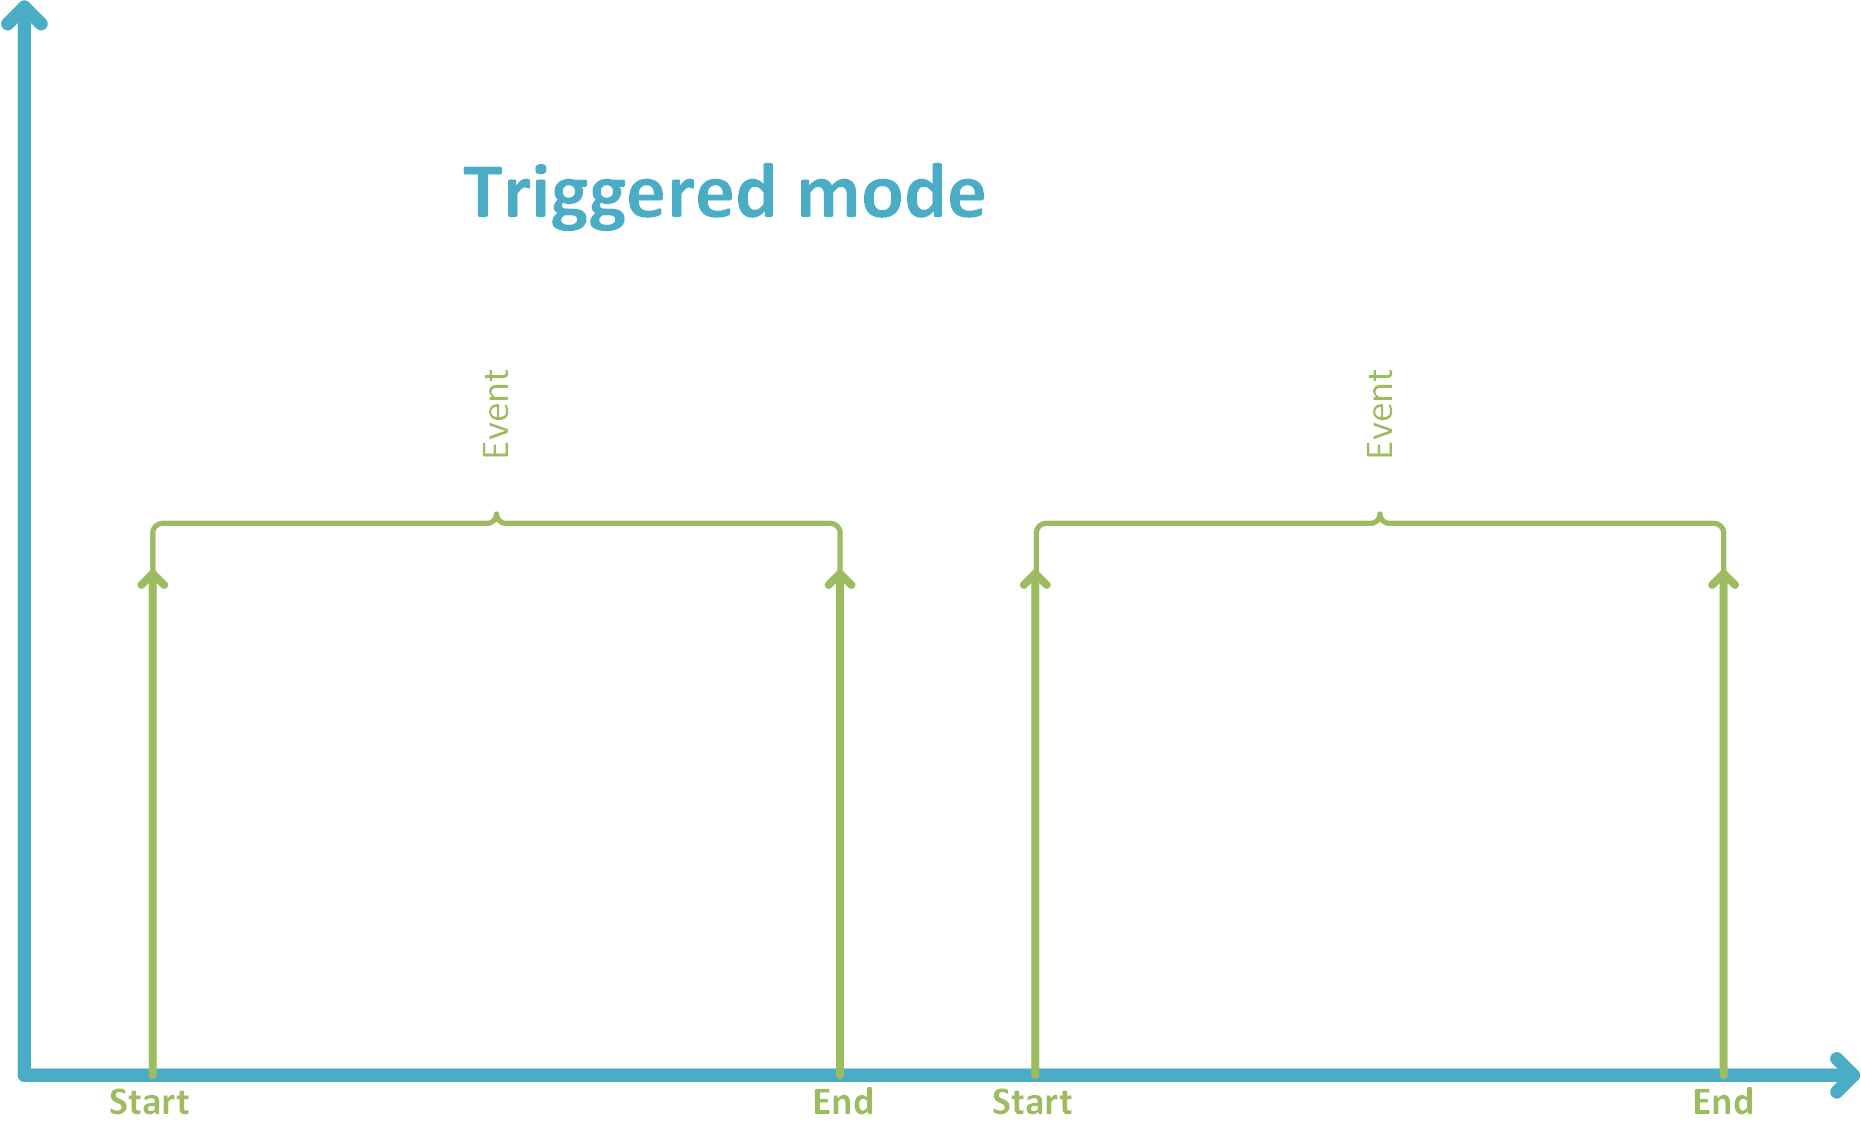
\includegraphics[width=\textwidth]{images/triggered-mode.png}
		\end{subfigure}
	\caption{Continuous vs Triggered mode}
	\label{fig:cont-vs-trig}
\end{figure}

\paragraph{}
The \gls{sampa} creates data packets from the data assembled from each time frame.
Consisting of a header of fixed size 50 bit, followed by a list of 10 bit samples, created from a single time frame.
Even though a time frame consists of 1024 clock cycles, in practice a maximum of 1022 samples are received each time.
This is due to the fact that 2 * 10 bit words are required to represent cluster size (size of consecutive samples) and a timestamp.
The headers are stored in their own \gls{fifo} buffers, separate for each channel, much like the sample buffers.
\ref{fig:packet} shows the structure and format of the packets.

\begin{figure}[h!]
	\centering
		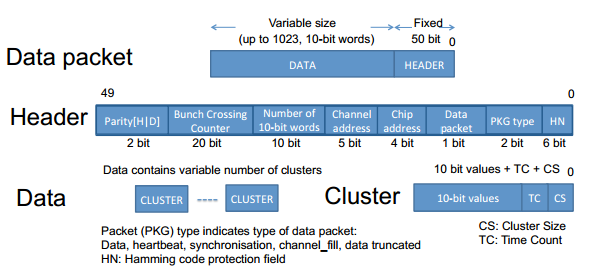
\includegraphics[width=1.0\textwidth]{images/packet.png}
		\caption{Data packet format \cite{tdr-015}}
		\label{fig:packet}
\end{figure}

\paragraph{}
The header consists of information regarding the data, such as address for the channel and chip, number of data words in the time frame and packet type.
The packet type is used as a marker to see if anything out of the ordinary has happened to the data.
This can be if there is no samples in the time frame, causing the packet type to just become a channel fill packet.
It can indicate if the stream of data was cut short because the \gls{fifo} buffer was full, causing buffer overflow.
In case of buffer overflow all data for the particular time frame are discarded and the empty packet is sent with type overflow.
Overflow can cause a lot of data to get discarded if the \gls{sampa} can't empty the buffers fast enough, this can happen if the buffers don't have enough space.
As the input rate is 3.2 Gbit/s and the readout speed is 1.28 Gbit/s, the \gls{sampa} can receive up to 2.5 times more data per second than it can pass along.
This is why the \gls{fifo} buffers are necessary, and finding a size which is sufficient, without giving overflow is crucial.

\paragraph{}
There have been done some calculations on how much data will actually be received from the detector at any given time.
It is estimated that on average over all channels for every \gls{sampa} there is around 30\% occupancy.
This means that on a global average there is 30\% data in every given time frame.
Some channels may be full while others are empty, and some may have 40\%, but on average there is 30\%, which means 306 samples out of 1022 for every time frame.
Taking this into account when calculating the input speed of the \gls{sampa} gives 960 Mbit/s which the design should be able to handle without any buffer overflow.
Even though there is an estimated average occupancy there can still be some channels which time frame after time frame gets a lot more then that, so how much can the design handle?
This is some of the question the simulation will give answers to.

\subsection{CRU}
The \gls{cru} serves as an interface between electronics directly on the detector and the online computing systems.
It is based on high performance \gls{fpga} processors, with optical fiber used as input and output \cite{tdr-015}. 
The \gls{cru} is somewhat out of the scope of the thesis, and will be regarded in the same fashion as the \gls{gbt}.
How the \gls{cru} is implemented in our design model has no effect on the tests which are going to be performed on the \gls{sampa} and its channels.
It is discussed in the thesis work of Damian K Wejnerowski, who is simulating the \gls{cru} and inspecting it in great detail.

\section{Signal processing in the SAMPA}
\paragraph{}
The \gls{sampa} chips will receive and process a huge amount of data, both relevant signals and background noise.
In section~\ref{subsec:sampa} we talked about occupancy and amount of samples in each time frame.
The estimated amount of 30\% refers to relevant samples, removing or compressing the background noise.
Seeing as it will always be some interference in the background, there will always come samples with data, and gathering all will be a waste of time and space that could be used on the actual collision data in the detector.
\ref{fig:signal} shows 2 actual events collected from the 2 different \gls{altro} channels, the events will look similar after the upgrade and we can use this as a starting point.
The x-axis expresses the current time bin within a time frame from 0 to 1021.
Here one can see that every sample in the time frame has some value most with 48-52, as well as certain peaks here and there.
Those peaks or pulses are what is interesting, everything else is considered noise and should be removed.
In order for any compression schema or method of reducing noise to be valid it needs to have a compression factor above 2.5 for the average amount of data being processed.
The compression factor will be the number of bits in a time frame before compressing compared to after. \codeword{factor = (bits before compression / bits after)}.
There are a number of ways to reduce the amount of noise, and/or compress the data to a manageable size.
What has been used with the current setup and is also discussed to use in in the upgraded setup is \gls{zs}.

\begin{figure}[t]
	\centering
		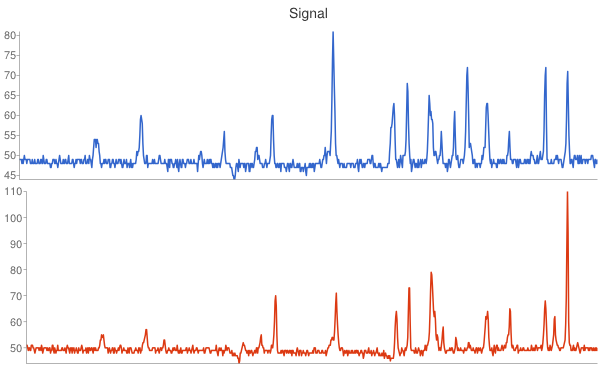
\includegraphics[width=1.0\textwidth]{images/signal.png}
		\caption{Two signals from a previous experiment}
		\label{fig:signal}
\end{figure}

\subsection{Zero suppression} 
\paragraph{}
\gls{zs} is the process of removing insignificant values below a set threshold or baseline.\cite{zerosuppression}.
Applying this in order to remove the background noise without discarding any important samples, a baseline for the \gls{zs} must be established.
The problem with this is that the baseline may shift, in the case of our 2 example time frames the first one has a visibly lower baseline by 1 or 2.
In the upgrade plans described in \cite{tdr-015}, it is specified how the signal processing will take place.
It works by looking at consecutive signals with value over the set threshold, confirming that the peak is indeed a real pulse.
The term real pulse refers to a sequence of signals over the threshold with more than one signal, standalone values over the threshold will be discarded.
The difference is displayed in \ref{fig:minseq}.

\begin{figure}[h!]
	\centering
		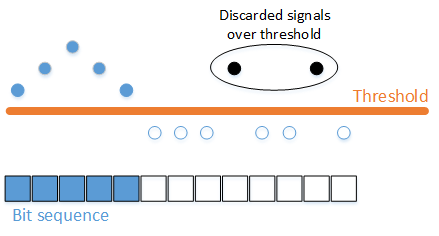
\includegraphics[width=0.75\textwidth]{images/minseq.png}
		\caption{Difference between a valid and invalid signal sequence.}
		\label{fig:minseq}
\end{figure}

\paragraph{•}
Because of the fact that \gls{zs} removes signals from various places in a time frame, the data losses its temporal positioning.
Therefore every real pulse must be tagged with a time stamp and a word representing the number of words in the pulse.
Since for every pulse we add two words, if two consecutive pulses are closer than three words they are merged and counted as one (\ref{fig:merge}).

\begin{figure}[h!]
	\centering
		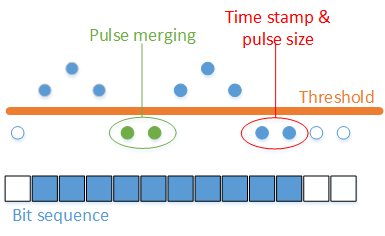
\includegraphics[width=0.75\textwidth]{images/merge.png}
		\caption{Merging of two pulses and the storing of extra pulse information.}
		\label{fig:merge}
\end{figure}

\paragraph{}
In some later discussion regarding the upgrade there has been questions if the described method is insufficient.
The theory behind the discussion is that the baseline will shift too much to be able to do efficient \gls{zs} without loosing important samples in the process.
Another argument against \gls{zs} is that with time frames with larger occupancies (40\%++) the compression factor is drastically reduced and will not be good enough.
This is because time frames with higher occupancy will have more signal pulses, and pulses will be closer together, meaning that more pulses will be merged rather than discarded. 
This encourage finding another way of processing the signals.
One proposed method is to use Huffman coding on the signal values.

\subsection{Huffman Coding} %Only real data
\paragraph{}
Huffman is a method used to achieve data compression\cite{huffman}.
It works by assigning binary codes to symbols in order to reduce the number of bits used to encode the symbol.
By looking at the frequency of appearance for every symbol used one can produce a frequency table sorted by most frequent.
One thing to note is that since the binary codes is of variable length, they may not all be uniquely decipherable.
For instance, if the codewords looks like the following: \codeword{\{0,01,11,001\}}, the code \codeword{0} is a prefix to \codeword{001}.
This is solved by using the right data structure to store the codes, the one most used is a \textit{full} \gls{bt}.
A \textit{full} \gls{bt} is a tree where every node either has zero or two child nodes.
The symbols are then generated by the path from the root to a leaf node, where left and right indicates 0 or 1.
\ref{fig:hm-ex} shows an example of a Huffman tree using made up frequencies for the letters A to D.
Here you can see the advantage of sorting by frequency, since the most frequent symbol A only needs one bit to store.
Creating the Huffman tree can be implemented using the following pseudo-code algorithm:

\begin{lstlisting}[caption=Huffman algorithm \cite{algorithms}, label=lst:huffman]
	//Input: An array f[1..n] of frequencies
	//Output: An encoding tree with n leaves
	//let H be a @\gls{pq}@ of integers, ordered by f
	function Huffman(f) {
		for(int i = 1; i <= n; i++){
			H.insert(i);
		}
		for(int k = n+1; k <= 2n - 1; k++){
			i = H.deletemin();
			j = H.deletemin();
			//Create a node numbered k with children i,j
			f[k] = f[i] + f[j];
			H.insert(k);
		}

	}
\end{lstlisting}

\begin{figure}[h!]
	\centering
		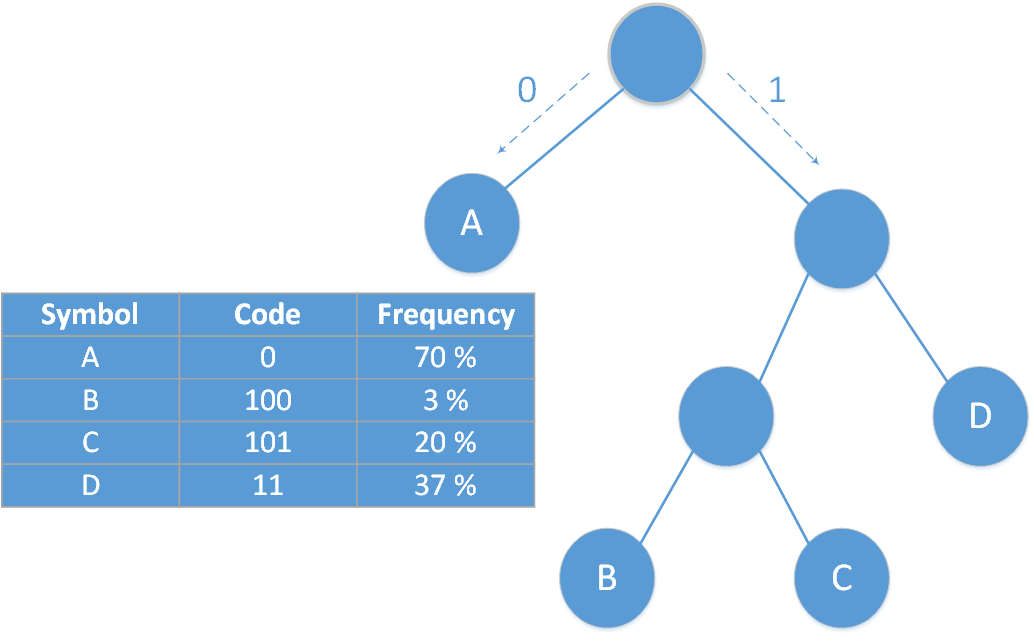
\includegraphics[width=1.0\textwidth]{images/huffman.png}
		\caption{Huffman tree with four symbols.}
		\label{fig:hm-ex}
\end{figure}

\paragraph{}
\textit{Need to have Dieter look over this paragraph}
In the context of compressing data coming from the detector there is one particular foreseen complication.
First of all, generating the Huffman tree needs values from the detector, so how do one create a tree with high compression factor without knowing this?
One answer to this is to generate a tree using existing data from previous experiments, but update the tree when receiving new data.
This gives us an uncertain compression factor in the beginning, but it will become better over time.
Because of a shifting baseline encoding the signal values directly may lead to a large Huffman tree, and the best tree for one channel may not be the same for another.
It is inefficient to create a separate tree for each channel, as there will be 160 channels for every \gls{fec}.
A possible solution to this is to encode the derivative of each signal in a time frame compared to the previous value.
In other words, for every signal \textit{n} you store the value: \textit{signal(n) - signal(n - 1)}.
Doing so takes away the problem caused by shift in the baseline as it only stores the difference between two signals.
This method requires that the first value of every time frame is stored somewhere(maybe the header of a \gls{sampa} packet) in order to decode it later on.


\paragraph{}
The way the \gls{fifo} buffers for each \gls{sampa} channel works is that it stores up to 10 bits in parallel for each slot.
This means that compressing 10 bit samples into smaller sizes will still take up 10 bit of space in the buffers. 
However reading the data from the buffer will be faster as there is less data to read.

\section{Designing the simulation model}
With all of the information regarding the different components already specified, creating a simulation model should be more than feasible.
There will be in total 3 main modules part of the simulation: the \gls{sampa}, \gls{gbt} and \gls{cru}, but focusing heavily on the \gls{sampa}.
In addition to the different modules there is need for a module which can be tasked with producing and/or distributing sample data to the simulation.
This module will contain all methods of sending samples to the different \gls{sampa} channels and in doing so start the entire simulation process.
The tasks, objectives and goals that this all boils down to is summarized in the list below.

\begin{itemize}
	\item \textbf{Tasks}
		\begin{itemize}
			\item Designing a model which is accurate, simple and customizable.
			\item Creating a data generator module which can send data to the simulation, both synthetic and real.
			\item Create a simulation test bench that allows for quick changes in order to run multiple simulations.
			\item Run different stress tests on the system, find out where it breaks and why.
			\item Run focused simulations on the \gls{sampa} channel buffers.
			\item Run simulations which compares \gls{zs} and Huffman encoding.
			\item Gather, and compile the simulation data into a readable and understandable format.
			\item Verify that the simulation results is comparable to what is expected, and calculated beforehand.
		\end{itemize}
	\item \textbf{Goals}
	\begin{itemize}
		\item With a verified simulation model, we have a created a strong argument that the results are valid.
		\item Find out how much \gls{sampa} buffer space is needed.
		\item Conclude the compression factor of both \gls{zs} and Huffman encoding.
		\item Verify the overall design of the \gls{sampa} chip, and use the results to come with a recommendation on possible changes.
	\end{itemize}
\end{itemize}

\section{Workflow}
Approaching this project, one must assume that there will be many uncertainties along the way.
Trying to simulate behaviour of an electronic system based solely on its early schematics, while others are working on the design in different areas will undoubtedly lead to many changes in the simulation model.
Another characteristic concerning this project is that it requires a lot of work before one can start to see any results, but after completing a satisfying  model the results should be easy to obtain without many changes to the simulation program.
Splitting the work into different phases, first a longer period of only working on the model, implementing the aspects that are known, and making the model ready to run simulations on.
When the base model is complete, an iterative process can start.
Simulate for a specific scenario, gather results from the simulation, compile it into a readable format, verify the correctness of the results, in the case they are not legitimate, make adjustments before running new simulations in the same scenario.
Customize the simulation parameters and tweak the model for different scenarios, and do the same as before.
This way any changes in requirements, or changes to the model can be handled in a separate iteration.
Working like this will result in a large period with no speakable results, but this will towards the end be very beneficial.

\chapter{Solution implementation}
\textit{Code snippets, Incremental implementation stages and the final implementation, (before and after huffman), using real data vs random. Implementing fluxiation into the simulation}
\section{Implementing the model in SystemC}
%Introduction
\subsection{The SAMPA module}

\paragraph{•}
As the focus of study in this project, the implementation of the \gls{sampa} is the most important piece to the simulation.
The overall structure to the \gls{sampa} consists of 32 channels, with a input port for each channel, and in total 4 serial outputs which reads data from the channel buffers.
There are a couple of things to think about when translating this design into code.

\begin{enumerate}
	\item What \gls{sc} channel should the input and output ports use.
	
		\begin{itemize}
		\item The requirements for the \gls{sampa} I/O ports is that everything comes in the correct order, and on a specific clock cycle.
		\gls{sc} comes with the channel type \codeword{sc\_fifo}, it contains both read and write methods, depending on what channel interface is implemented.
		So for our one directional design this should work perfectly.
		The clock cycle is not tied to the ports specifically and will be handled separately.
		\end{itemize}	
		
	\item What data structure to use for the channel buffers.
		\begin{itemize}
\item When choosing a data structure one need to think about what the purpose of it is, what operations are being done on it, and so forth.
		The essential attributes the structure must have are: \textit{Insert} items to the back, \textit{Read/Remove} items from the front, dynamical storage space, and the structure should be a linear one-dimensional sequential storage.
		On first glance using a \gls{fifo} like structure sounds like the best way to go.
		However in addition to the essential attributes it may be needed to be able to remove and read from the back of the buffer.
		This is because in the simulation it can be used to grab statistical data from the buffer, and reading from the back will not have any impact of the simulation result, but can make the buffers more versatile.
		\gls{cpp} has many different data structures to choose from, all depending on the need for it.		
		In \ref{tab:ds} three different \gls{cpp} data structures are being evaluated: \codeword{vector}, \codeword{list} and \codeword{queue}.
		From this table and the requirements of what is needed from the buffer structure, it becomes clear that the \codeword{list} container has all the attributes needed, as well as performing equally or better than the rest in the different operations.
\end{itemize}
		
	
	\item Handling the clock frequency.
		\begin{itemize}
		\item \gls{sc} will handle the clock frequency for us, the only thing to note is that \gls{sc} uses pauses in the threads as a way to simulate the clock cycles.
		In other words, one perform the actions for 1 clock cycle, than the wait statement, and repeat.
		This means that the frequencies need to be converted to a time delay.	
		An example of such a conversion is shown in listing~\ref{lst:cons-ex}.
		\end{itemize}	
	
\end{enumerate}

\begin{table}
\begin{tabular}{| l | l | l | l | p{6cm} |}
\hline
 & \multicolumn{3}{c |}{\textbf{\large{Time}}} & \\
 \hline
\textbf{Operation} & \textbf{Vector} & \textbf{List} & \textbf{Queue} & \textbf{Remarks} \\
\hline
Add back & O(1) & O(1) & O(1) & Constant time for all containers.\\
\hline
Add front & O(n) & O(1) & X & Vector does not have a direct method for adding to front. Queue cant do that at all.  \\
\hline
Access back & O(1) & O(1) & O(1) & Constant time for all containers.\\
\hline
Access front & O(1) & O(1) & O(1) & Constant time for all containers.\\
\hline
Remove front & O(n+m) & O(1) & O(1) & Vector erase is linear to number of deleted elements + number of elements after last deleted item (moving). \\
\hline
Remove back & O(1) & O(1) & X & Queue does not have a method for doing this.\\
\hline
Size of container & O(1) & O(1) & O(1) & Constant time for all containers.\\
\hline

\end{tabular}
\caption[Data structure comparison.]{Data structure comparison\cite{vector}, \cite{list}, \cite{queue}.}
\label{tab:ds}
\end{table}

\paragraph{•}
One possible setup for the \gls{sampa} deceleration is shown in listing~\ref{lst:sampa1}.
This takes everything we need into account, storing the channel header and data buffer in an array, declaring input ports, and the output elinks.
In addition it declares a single thread for receiving signals, and four threads representing the serial outs reading from the channel buffers.
Lets now look at how the implementation for receiving signals can look like.
In listing~\ref{lst:sampa1.2} the thread logic is implemented, and here some weaknesses with the \gls{sampa} module becomes clear.
Having to iterate over every channel every timebin can become costly and hard to maintain when the code becomes more complex.
In the code shown there is already a flaw, if one of the channel buffers has \codeword{overflow}, none of the other buffers will receive data.
The \codeword{overflow} variable needs to be stored as a array as well to be able to know what channel it represented.
The same problem will occur for every value that is unique for each channel.
A principle of \gls{oop} is single-responsibility, meaning that every class/object should be responsibly for one piece of functionality.
One solution to the previous problem following this principle can be to create a \codeword{Channel} sub-module inside of the \gls{sampa} module.
The channel module will contain logic for receiving signals, as this happens for every channel, while the \gls{sampa} will contain the serial outs, which are accessing data from the buffers.

\begin{minipage}{\linewidth}
\lstinputlisting[caption=SAMPA - First iteration.,firstline=1,lastline=25,label=lst:sampa1]{codelistings/sampa1.cpp}
\end{minipage}

\begin{minipage}{\linewidth}
\lstinputlisting[caption=Receive thread.,firstline=27,lastline=53,label=lst:sampa1.2]{codelistings/sampa1.cpp}
\end{minipage}

\paragraph{•}
The changes made to the \gls{sampa} and \codeword{Channel} modules is shown in listing~\ref{lst:sampa2} and \ref{lst:channel1}.
The \gls{sampa} now has an array of \codeword{Channel} modules, a new method called \codeword{initChannel()} that initiate the channels, and connects them to the correct input port.

\begin{minipage}{\linewidth}
\lstinputlisting[caption=SAMPA - Second iteration.,firstline=1,lastline=26,label=lst:sampa2]{codelistings/sampa2.cpp}
\end{minipage}

\begin{minipage}{\linewidth}
\lstinputlisting[caption=Channel module.,firstline=1,lastline=24,label=lst:channel1]{codelistings/channel.cpp}
\end{minipage}

The \codeword{Channel} module now has the \codeword{receiveData()} thread, and its own data/header buffer.
Having it structured like this makes it possible to add \codeword{Channel} specific variables or methods, without disturbing the \gls{sampa} as a whole.
The implementation of the receive thread is now more simple in terms of complexity, and is exclusive for each \codeword{Channel}.
Listing~\ref{lst:receive-channel} shows the basic thread structure, excluding any data compression or processing.
It continuously receives samples and adds them to the buffer, unless the buffer reach its maximum size.

\begin{minipage}{\linewidth}
\lstinputlisting[caption=Receive samples.,firstline=26,lastline=62,label=lst:receive-channel]{codelistings/channel.cpp}
\end{minipage}


\paragraph{•}
The basic implementation of reading from the buffer is somewhat more complicated than receiving data.
This is because the real reading procedure is more complex in itself.
In listing~\ref{lst:read-buffers} the procedure is shown, along with one of four equal serial out threads.
The procedure loops through the eight channels for the given serial out, getting the correct channel, and reading out the entire timeframe.
One thing to notice here is that the actual data from the buffers aren't passed along further.
This is because we only care about the time it takes to transfer them, which is being calculated in the \codeword{wait} statement.
The header packet is sent as it contains important information which can be useful later on.

\begin{minipage}{\linewidth}
\lstinputlisting[caption=Reading data from the SAMPA buffers.,firstline=28,lastline=72,label=lst:read-buffers]{codelistings/sampa2.cpp}
\end{minipage}

\paragraph{•}
The implementation of the \gls{zs} and the Huffman procedures will be discussed in a later section.

\subsection{The DataGenerator module}
\paragraph{•}
The simulation model is scoped to the readout electronics, which doesn't handle the creation of signals.
This means that the simulation needs a module which can create and distribute data, both simulated and real to the \gls{sampa} modules.
The module needs to be able to continuously send samples based on what is desired for a specific simulation scenario.
It is important that all the different methods for sending samples, do so in the same fundamental way.
The rest of the simulation model should not need to change for each different scenario, but instead the data generator should make sure that it sends samples in the correct format, regardless of the simulation type.

\paragraph{•}
With the expected behaviour given in the previous paragraph, the bounds and requirements of the data generator can be established.
The module will continually be updated, and new functionality will be added as new simulation scenarios (surface?). 
In order for this to be efficient, the module needs to be easily extended, without causing any disturbance to the rest of the module.
Sending samples should follow the specifications for the actual hardware, emulating the connection between the readout chambers and the \gls{sampa} asic.


\subsection{Signal classes}
\paragraph{•}
\gls{sc} allows the creation of custom \codeword{classes} to be used as data type when transferring data between modules.
There are some requirements when doing so that needs to be fulfilled for it to work.
\gls{sc} requires you to define several methods which is vital for the read/write methods of a \gls{sc} channel.
The read/write methods involve copying the custom data type.
Because of this it requires the definition of the assignment operator(\codeword{operator=()}).
In addition the output streaming(\codeword{ostream\& operator<<()}) method is required. 

\paragraph{•}
The simulation needs two different data types, these have been briefly shown in the previous code listings.
The \codeword{Sample} and the \codeword{Packet} classes.
\codeword{Sample} represents a single 10-bit signal, storing information about what timeframe the sample belongs to, the signal value itself, and other statistical variables.
Representing the \gls{sampa} header is the \codeword{Packet} class, it stores the relevant values selected from its documentation.
This include the timeframe, channel id, sampa id, number of samples and whether there was overflow in its timeframe.
Source code for the \codeword{Packet} class is shown in listing~\ref{lst:packet}.
The \codeword{Sample} class is implemented in similar fashion and will not be displayed in the report. 

\begin{minipage}{\linewidth}
\lstinputlisting[caption=Custom data type - The SAMPA header.,label=lst:packet]{codelistings/packet.cpp}
\end{minipage}

\subsection{Lesser modules}
\subsection{Connecting the modules together}
\section{Creating a customizable testbench}
\section{Data gathering}

\chapter{Evaluation and results}
\textit{Running the tests, results from different tests, Evaluating the final product}
\section{Simulation results}
\subsection{Initial test scenarios}
\subsection{First substantial simulations}
\subsection{Full simulation}

\subsection{Zero Suppression - preliminary results}
\subsection{Zero Suppression - extended results}
\subsection{Huffman results}

\chapter{Conclusion and Future work}
\textit{Conclude the thesis, talk about the impact it has and its usefulness in future planing of the front end electronics.}

\bibliography{biblio}{}
\bibliographystyle{unsrt}
\end{document}
